%===============================================================================
% Template Name:      SUnORE Starter Presentation template
% Template URI:       http://sunore.co.za/sunore-presentation/
% Description:        Starter Presentation template for SUnORE
%                     Department of Industrial Engineering,
%                     Stellenbosch University
% Version:            1.1.0
% Author:             Johan Janse van Rensburg
% Author URI:         http://johanjvrens.co.za/
% License:            MIT License
% License URI:        http://opensource.org/licenses/MIT
%===============================================================================
\documentclass[helvetica,11pt]{beamer}

%=================================================
% theme and color
%=================================================
% \usetheme{metropolis}
\usecolortheme[snowy]{owl}

%=================================================
% packages and new commands
%=================================================
\usepackage[ruled, linesnumbered, vlined]{algorithm2e}
\usepackage{epsfig, subfigure, amssymb, multirow, algorithmic, amsmath}
\usepackage{listings}
% \usepackage{harvard}
% \usepackage{natbib}
\usepackage{xcolor}

\lstset{%
    %backgroundcolor=\color{yellow!20},%
    basicstyle=\footnotesize\ttfamily,%
    }%

% Add your keywords here, and have this in a separate file
% and include it in your preamble
\lstset{emph={%
    global, protocol, from, to, choice%
    },emphstyle={\color{blue}\bfseries}%
}%
\newcommand*{\superscript}[1]{\ensuremath{^{\rm #1}}}
\newcommand*{\subscript}[1]{\ensuremath{_{\rm #1}}}
\newcommand\blfootnote[1]{%
  \begingroup
  \renewcommand\thefootnote{}\footnote{#1}%
  \addtocounter{footnote}{-1}%
  \endgroup
}

%=================================================
% thesis details (preamble)
%=================================================
\title[{\sc Session Types in the Wild } \hspace{0.8cm} \insertframenumber/\inserttotalframenumber]{{\sc Session Types in the Wild}}
\author[Viva --- {\sc Jun 15\superscript{st}, 2017}]{{A. Laura Voinea}}
\date{15 Jun 2017}
% \institute{School of Computing Science\\ University of Glasgow, UK}
\institute{First supervisor: Simon Gay\\ Second supervisor: Wim Vanderbauwhede}

%=================================================
% start presentation
%=================================================
\begin{document}

%========================
% title page
%========================
\begin{frame}
  \begin{center}
    \vspace{0.1cm}
    \includegraphics[scale=0.65]{compsci_logo.pdf}
  \end{center}
  \titlepage
% \blfootnote{Funded by UK EPSRC grant “From
%   Data Types to Session Types: A Basis for Concurrency and
%   Distribution” (EP/K034413/1) (Simon Gay, Phil Wadler and Nobuko Yoshida)}
\end{frame}

%========================
% your slides:
%========================
\label{thesis}
\begin{frame}\frametitle{Thesis Statement}
    Data types and typing theories have proved to be essential for sequential computation. The session control and discipline that session types provide are  similarly important for concurrent, distributed programming. To further incorporate session typing in practical settings, we must be able to express subtle and complex protocols and make safety guarantees. While providing strong guarantees, linearity is often an obstacle for expressivity. Specifying protocols without the full cost of linearity, without sacrificing safety would be highly beneficial.
\end{frame}

\begin{frame}\frametitle{Session Types: Intro}
What are Session Types?
\begin{itemize}
\item Type discipline for specifying protocols in communication-intensive systems(e.g. multi-core programming, mobile applications, or web services)
% \item Formalism to model protocols in distributed systems
\item Introduced more than 20 years ago by~\cite{honda93, takeuchi94, honda98}
\item Guarantee properties such as privacy, communication safety and session fidelity
\item At runtime communication follows the protocol
\item Significant theme in programming languages
\end{itemize}

\end{frame}

\begin{frame}\frametitle{Session Types: Example}

  \begin{figure}[htb]
    \centering
    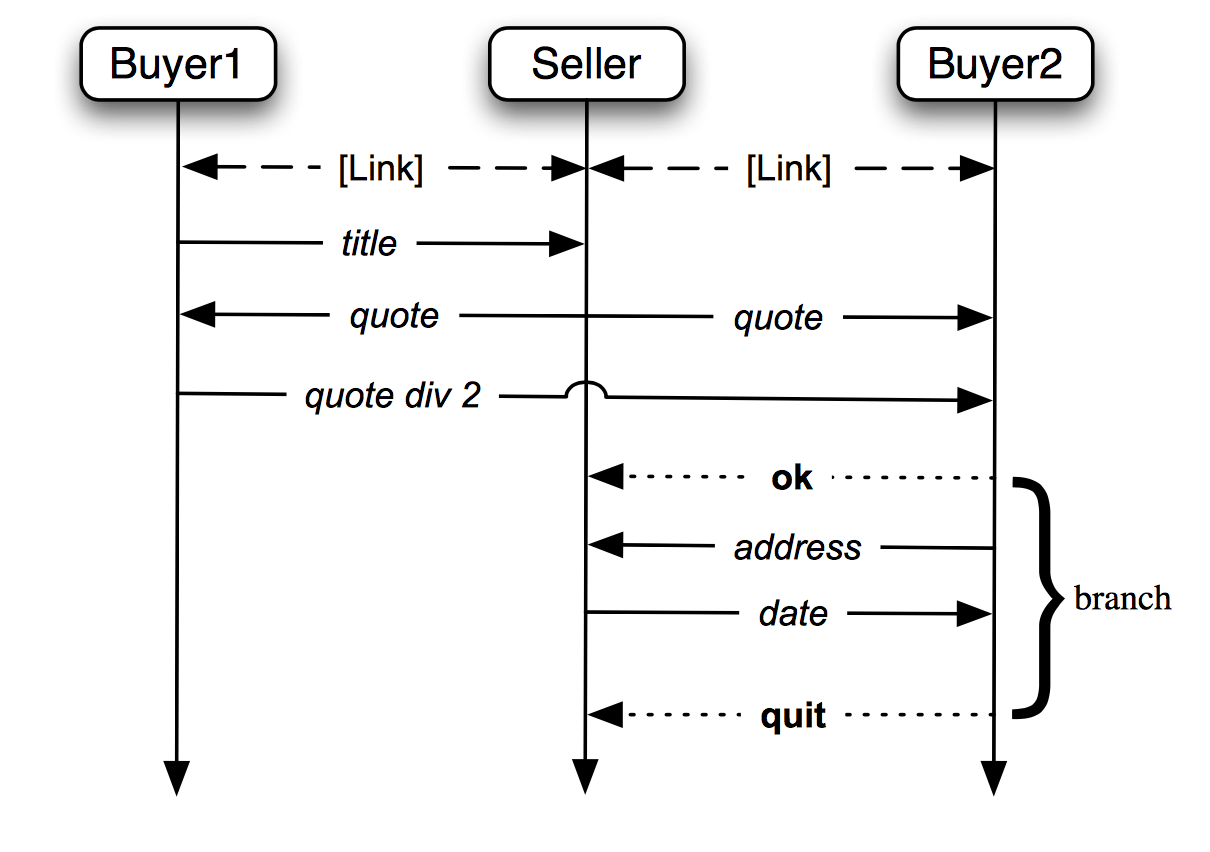
\includegraphics[scale=0.45]{examples/TwoBuyer.png}
    \caption{Two Buyer Protocol~\cite{honda2008multiparty}}
  \end{figure}
\end{frame}
%First Buyer1 sends a book title to Seller, then Seller sends back a quote to Buyer1/2; Buyer1 now tells Buyer2 how much she can contribute, and Buyer2 notifies Seller if it accepts the quote or not.

\begin{frame}[fragile]\frametitle{Session Types: Example}
  \begin{lstlisting}
  global protocol TwoBuyer(role Buyer1, role Buyer2,
  role Seller) {
    book(title) from Buyer1 to Seller;
    book(quote) from Seller to Buyer1, Buyer2;
    contribution(quote) from Buyer1 to Buyer2;
    choice at Buyer2 {
      ok from Buyer2 to Seller;
      deliver(address) from Buyer2 to Seller;
      deliver(date) from Seller to Buyer2;
      } or {
      quit from Buyer2 to Seller;
      }
      }
  \end{lstlisting}\footnote{written in Scribble, a protocol description language that can describe how two or more participating entities interact should interact with each other \url{www.scribble.org}}
  ~\cite{honda2008multiparty}
\end{frame}

% \begin{frame}\frametitle{Mungo I}
%
%   \begin{alertblock}{Mungo Background}
%   \begin{itemize}
%     \item Java front-end tool, developed at the University of Glasgow
%     \item Statically checks the order of method calls
%     \item A session type is represented as a typestate protocol in a separate file, associated with a Java class.
%     \item The protocol definition is described as a sequence of method calls, the order of which determines the validity of the protocol.
%   \end{itemize}
% \end{alertblock}
% \end{frame}
%
%
% \begin{frame}\frametitle{Mungo II}
%
% \begin{alertblock}{Research Activities}
%   \begin{itemize}
%     \item Ported the tool to a new compiler framework \hfill \textit{year 1}
%     \item Support  for annotations  \hfill   \textit{year 1 + 2}
%     \item Syntactic support for generic types  \hfill  \textit{year 2}
%     \item Typestate annotation, through which typestate
%   specifications are associated with Java classes  \hfill  \textit{year 2}
%     % \item Update repositories \hfill   \textit{ongoing}
%     \item Typecheck exceptions  \hfill  \textit{ongoing}
%     \item Typecheck generic types \hfill   \textit{ongoing}
%   \end{itemize}
% \end{alertblock}
% \end{frame}
%
% \begin{frame}\frametitle{Mungo III}
% \begin{alertblock}{Further Research}
%   \begin{enumerate}
%   \item Typecheck collections
%   \item Explore a new concept of context-free typestates
%   \item Flexible aliasing
%   \item Research/implement new features and issues that may arise
% \end{enumerate}
%
% \end{alertblock}
%
% \end{frame}


\begin{frame}\frametitle{Paxos + Mungo}
  \begin{alertblock}{Paxos}
    \begin{itemize}
      \item Solving consensus in a network of unreliable processes
      \item Provably correct, and non-blocking if a majority of participants are available
      \item Implemented in the session type system for unreliable broadcast communication devised by Gutkovas, Kouzapas, and Gay
    \end{itemize}
  \end{alertblock}
  \begin{alertblock}{Mungo}
    \begin{itemize}
      \item Java front-end tool, developed at the University of Glasgow
      \item Statically checks the order of method calls
      \item A session type is represented as a typestate protocol in a separate file, associated with a Java class
      % \item The protocol definition is described as a sequence of method calls, the order of which determines the validity of the protocol.
    \end{itemize}
  \end{alertblock}

\end{frame}

\begin{frame}[allowframebreaks]\frametitle{StMungo}

  \begin{alertblock}{StMungo Background}
  \begin{itemize}
    \item Java-based tool developed at the University of Glasgow
    \item translates a Scribble local protocol to a Mungo specification and skeleton socket-based implementation code
  \end{itemize}
\end{alertblock}


\begin{alertblock}{Development}
  \begin{itemize}
    \item Additional Scribble constructs: no payload, multiple payload, messages without a signature, annotated payloads \hfill  \textit{year 1}
    \item Various convenience features \hfill  \textit{year 1}
    \item Special cases of recursion and choice \hfill  \textit{year 1}
    \item Collaborated with Florian Weber on a plug-in for mapping between concrete and abstract messages from Scribble to the `real-world' representation
    \hfill  \textit{year 2}
    \item Translate inlined protocols and sub-protocols \hfill  \textit{ongoing}
    \item Keep up to date with in Scribble and Mungo \hfill  \textit{ongoing}

  \end{itemize}
\end{alertblock}

\begin{alertblock}{Further Development}
  \begin{enumerate}
    \item Support more complex constructs such as interruptible or parallel
\end{enumerate}

\end{alertblock}


\end{frame}

\begin{frame}\frametitle{Language evaluation}
  \begin{alertblock}{Usecases}
  \begin{itemize}
    \item File Transfer Protocol (FTP) \hfill  \textit{year 1 + on hold}
    \item Paxos \hfill  \textit{year 1 + 2}
  \end{itemize}
\end{alertblock}


\begin{alertblock}{User Studies}
  \begin{itemize}
    \item preliminary literature review \hfill  \textit{year 1 + 2}
    \item preliminary hypotheses work \hfill  \textit{year 2}
    \item Mungo toolset experiment plan \hfill  \textit{year 1 + 2}
    \item conduct Scribble experiment \hfill  \textit{year 3}
    \item conduct Mungo experiment \hfill  \textit{year 3}
  \end{itemize}
\end{alertblock}

\end{frame}


%\subsection{Figures}
\newcounter{loopcntr}
\newcommand{\rpt}[2][1]{%
  \forloop{loopcntr}{0}{\value{loopcntr}<#1}{#2}%
}
\newcommand{\on}[1][1]{
  \forloop{loopcntr}{0}{\value{loopcntr}<#1}{&\cellcolor{blue}}
}
\newcommand{\off}[1][1]{
  \forloop{loopcntr}{0}{\value{loopcntr}<#1}{&}
}
\newcommand{\onx}[1][1]{
  \forloop{loopcntr}{0}{\value{loopcntr}<#1}{&\cellcolor{cyan}}
}

\label{figures2}
\begin{frame}\frametitle{Work Plan}
  \noindent\begin{tabular}{p{0.08\textwidth}*{16}{|p{0.019\textwidth}}|}
  % The top line
  Task
             & \multicolumn{7}{c|}{2018}
             & \multicolumn{9}{c|}{2019}\\
  % The second line, with its five years of four quarters
  % \rpt[2]{& 1 & 2 & 3 & 4} \\
  & 06 & 07 & 08 & 09 & 10 & 11 & 12
  & 01 & 02 & 03 & 04 & 05 & 06 & 07 & 08 & 09\\

  \hline
  % using the on macro to fill in twenty cells as `on'

  A  \on[3] \off[13] \\
  \hline
  B \on[5] \off[11]\\
  \hline
  C \off[5] \on[4] \off[7] \\
  \hline
  D  \off[6] \on[4] \off[6]\\
  \hline
  \end{tabular}
  \begin{enumerate}[A]
  \item Modular linearity with Capabilities
  \item Semantic approach to modular linearity
  \item Paxos \& Mungo
  \item Thesis write-up
  \end{enumerate}
\end{frame}

% \begin{frame}\frametitle{Conclusion}
% \begin{itemize}
%   % \item Session Types are a very simple but powerful formalism to model protocols in distributed systems
%   \item Plenty of scope to study the impact of session type design
%   \item Many interesting questions
%
%   \item different tools and implementations for the same language with no comparison between them
% \end{itemize}
%
% \textbf{Goal:} Improve session types by identifying which designs and implementations help or hinder programmers
%
% \end{frame}

\begin{frame}[fragile]\frametitle{Q\&A}
  \begin{lstlisting}
  global protocol Q&A(role you, role me) {
    rec Loop
    {
        question(question:String) from you to me;
        answer(answer:String) from me to you;
        continue Loop;
    }
  }
  \end{lstlisting}
  %\footnote{written in Scribble, a protocol description language that can describe how two or more participating entities interact should interact with each other \url{www.scribble.org}}

\end{frame}


\begin{frame}\frametitle{Modular linearity with Capabilities -- Typing Rules}
  \begin{figure}
  \tiny{
    \[
    \arraycolsep=0pt
    \begin{array}{ll}
    \tree{
    % \\
    }{
      \Delta; \Gamma , x: T \types x: T
    }{}{\TVar}

    \qquad
    \tree{
    % \\
    }{
      \Delta; \Gamma , x: tr(\rho_x) \types x: tr(\rho_x); \{\rho_x \mapsto S\}
    }{}{\TVar}
    \\ \\
    \tree{
    \Delta; \Gamma
    \andalso
      v \in T
    }{
      \Delta; \Gamma \types v: T, C
    }{}{\TVal}

    \qquad


    \tree{
    C \text{ completed}
    }{
    \Delta; \Gamma \types \nil; C
    }{\TInact}

    \\ \\

    \tree{
    \Delta; \Gamma \types P; C_P
    \andalso
    \Delta; \Gamma \types Q; C_Q
    }{
      \Delta; \Gamma \types P \pll Q; C_P \otimes C_Q
    }{}{\TPar}

    \qquad

    \tree{
      \Delta; \Gamma \types x: Bool \andalso \Delta; \Gamma \types P; C \andalso \Delta; \Gamma \types Q; C
    }{
      \Delta; \Gamma \types \cond{x}{P}{Q}; C
    }{}{\TCond}
    \\ \\
     \tree{
       \Delta; \Gamma, x: tr(\rho_x), y: tr(\rho_y) \types P; C \otimes \{\rho_x \mapsto S\} \otimes \{\rho_y \mapsto \tdual S\}
     }{
       \Delta; \Gamma \types \newn{xy} P; C_P
     }{}{\TRes}

     \\ \\

      % \qquad


      \tree{
      \Delta, \rho_y; \Gamma, x : tr(\rho_x), y: tr(\rho_y) \types P; C \otimes \{\rho_x \mapsto U\} \otimes \{\rho_y \mapsto S\}
        }{
          \Delta; \Gamma, x: tr(\rho_x) \types \pin{x}{y} P; C \otimes \{\rho_x \mapsto \forall [\rho_y].\tin S U \}
        }{\TRcv}

        \\ \\
        \tree{
        \Delta; \Gamma, x : tr(\rho_x), y: T \types P; C \otimes \{\rho_x \mapsto U\}
          }{
            \Delta; \Gamma, x: tr(\rho_x) \types \pin{x}{y} P; C \otimes \{\rho_x \mapsto \tin T U \}
          }{\TRcvVal}
      % \qquad

      \\ \\
      \tree{
      \Delta, \rho_v; \Gamma, x: tr(\rho_x) \types P; C \otimes \{ \rho_x \mapsto U\}
        \andalso
      \Delta; \Gamma \types v : tr(\rho_v); \{\rho_v \mapsto S\}
      }{
      \Delta; \Gamma, x: tr(\rho_x) \types \pout{x}{v} P; C \otimes \{\rho_x \mapsto  \forall [\rho_v].\tout S U\} \otimes \{\rho_v \mapsto S\}
      }{\TSnd}
      \\ \\
      \tree{
      \Delta; \Gamma, x: tr(\rho_x) \types P; C \otimes \{ \rho_x \mapsto U\}
        \andalso
      \Delta; \Gamma \types v : T
      }{
      \Delta; \Gamma, x: tr(\rho_x) \types \pout{x}{v} P; C \otimes \{\rho_x \mapsto  \tout T U\}
        }{\TSndVal}
    \\ \\
    % \qquad

      \tree{
      \Delta; \Gamma, x: tr(\rho_x) \types P; C \otimes \{\rho_x \mapsto S_j\}, j \in I
      }{
      \Delta; \Gamma, x : tr(\rho_x) \types \sel{x}{\ell_j} P; C \otimes \{\rho_x \mapsto \tselI{\ell}{S}\}
      }{\TSel}


      \\ \\
      \tree {
      \Delta; \Gamma, x : tr(\rho_x) \types P_i; C \otimes \{\rho_x \mapsto S_i\}, \forall i \in I
      }{
        \Delta; \Gamma, x : tr(\rho_x) \types \branch{x}{\ell_i:P_i}_{i \in I}; C \otimes \{\rho_x \mapsto \tbranchOn{\ell_i:S_i}_{i \in I}\}
      }{\TBr}
    \end{array}
    \]
    }
  \end{figure}
\end{frame}

\begin{frame}\frametitle{Example -- Addition server}

  Type: $ S = \tin \tint \tin \tint \tout \tint \tend $


  Process: $ server(x) = \pin{x}{int} \pin{x}{int} \pout{x}{int} \nil $

  Let $\Theta = \Delta; \Gamma, x: tr(\rho_x)$ and $c = a + b$.
  \begin{figure}[H]
    \noindent
  $
  % \infrule{
    % \infrule{
      % \infrule{
      %   \Theta \types \nil; C \otimes \{ \rho_x \mapsto U\}
      %     \quad

        \infrule{\Delta; \Gamma}
                {\Delta; \Gamma \types c: \tint}{\TVal}
        % }{\Theta, c: \tint \types \pout{x}{c} \nil; C \otimes \{\rho_x \mapsto \tout \tint U\}}\rulename{\TSndVal}
        % \quad
        % \infrule{\Delta; \Gamma}
        % {\Delta; \Gamma \types b : \tint}{\TVal}
        % }{\Theta, a : \tint \types \pin{x}{b} \pout{x}{c} \nil; C \otimes \{\rho_x \mapsto \tin \tint U\}}\rulename{\TRcvVal}

    %
    % \quad
    % \infrule{\Delta; \Gamma}
    % {\Delta; \Gamma \types a : \tint}\rulename{\TVal}
    % }
    % {\Theta \types \pin{x}{a} \pin{x}{b} \pout{x}{a+b} \nil; C \otimes \{\rho_x \mapsto \tin \tint U\}}\rulename{\TRcvVal}
  $

%   \caption{}
%   \label{}
% \end{sidewaysfigure}
\end{figure}

\end{frame}

% % \begin{frame}\frametitle{Mungo}
%
% • Mungo is a Java front-end tool that statically checks the order of method calls.
% • It is based on the notions of typestate – describing non-uniform objects– and session types – describing a protocol on the method calls.
% • A Java class is augmented with a typestate. Mungo checks that method calls follow the declared typestate of an object.
% • Contributors: ABCD Glasgow team.
% • Link: http://www.dcs.gla.ac.uk/research/mungo/
% \end{itemize}
% \end{frame}

\begin{frame}\frametitle{What next?}
  \begin{itemize}
    \item Design and carry out experiments
    \item Investigate with H1 and H2 in various contexts
    \item Start with Java, popular mainstream language, and Mungo, Java based tool at Glasgow University
  \end{itemize}

  Mungo:
  \begin{itemize}
    \item Java front-end tool, developed at the University of Glasgow
    \item Statically checks the order of method calls
    \item A protocol or session type is represented as a separate typestate file, associated with a Java class.
    \item The protocol definition is described as a sequence of method calls, the order of which determines the validity of the protocol.

  \end{itemize}
\end{frame}


\begin{frame}[fragile]\frametitle{Proposed experiment}
% Null hypothesis: Usually a neutral statement stating that
% groups are not different (e.g., novices using a particular
% language will perform equally)
%
%
% Alternative hypothesis: Usually the opposite of the null
% hypothesis (e.g., novices using a particular language will
% perform better than another)
%
% Experimental design:
%
% Considering that the aim of this experiment is exploratory and the learning effect (performance improving with experience, even over very short periods of time) is of little concern in this case a within subjects design, every participant perform every task under every condition, will be used.
\textbf{Investigate how programmers work with Mungo.}\\
Tasks:
\begin{itemize}
  \item Modify an existing and debug a program (such as POP3);
  \item Starting from an English description code Iterator, Fibonacci, Two Buyer Protocol\\
\end{itemize}
Measurements:
\begin{itemize}
  \item time to complete each task, order in which tasks are performed, how many times the code is compiled, how many bugs/errors, is the end result correct, personal experience\\
\end{itemize}
Subjects:
\begin{itemize}
  \item 4th year computer science students\\
\end{itemize}
%
% the experimental design (e.g. AB experiments, repeated measures, Solomon 4-group designs),
% • the experimental unit (e.g. the concrete source code to be modified or to be written),
% • the measurement (e.g. time required to solve a problem),
% • the subjects (e.g. children, first year college students,
% professionals),
% • the sample size (e.g. 42 subjects)
% • the analysis technique (e.g. T-Test, structural equation modeling),
% • the effect size of the technique or the approach to be tested (so-called variance accounted for),
% • the conclusion step (e.g. alpha-level of .05), and
% • Threats to validity (e.g., non-standard experimental de-
% signs, missing data).

\end{frame}



  % Sample size:
  % Analysis technique:
%   Null hypothesis: Usually a neutral statement stating that
%   groups are not different (e.g., novices using a particular
%   language will perform equally)
%
%
%   Alternative hypothesis: Usually the opposite of the null
%   hypothesis (e.g., novices using a particular language will
%   perform better than another)
%
% Experimental design: AB experiment/Within-subjects designs:
% 20 minute tutorial on Session types
%
% Tasks:
% Measurements: time to complete each task, how many times the code is compiled, how many bugs/errors, is the end result correct
% Subjects: Computer scientists with Java experience
% Sample size:
% Analysis technique:

% \begin{frame}[allowframebreaks] \frametitle{Hypotheses}
% \begin{enumerate}
% \item Programming with session types can be understood and used efficiently by real world programmers.
% \item Programming with session types improves \textbf{software reliability}.
% \item Session types improve source \textbf{code readability}.~\cite{yoshida07,vasco09,kouzapas16} \url{www.scribble.org}
% \item Session types promote \textbf{modular programming}.~\cite{yoshida07,kouzapas16} \url{www.scribble.org}
% \item Session types can help increase \textbf{software maintainability}.~\cite{yoshida07,yoshida07,kouzapas16} \url{www.scribble.org}
% \item Session typed make \textbf{debugging faster} and more precise.~\cite{yoshida07,vasco09,kouzapas16} \url{www.scribble.org}
% \item Programming with session types speeds up the \textbf{development process}.~\cite{yoshida07,abcd} \url{www.scribble.org}
% \item Programming with session types improves \textbf{software efficiency}~\cite{mostrous2007two}; Tytra:Exploiting {P}arallelism through {T}ype {T}ransformations for {H}ybrid {M}anycore {S}ystems(Professor N	Gay Yoshida, Professor SJ	Gay, Professor S Scholz, Professor W Luk).
% \end{enumerate}
%
% \end{frame}

\begin{frame}\frametitle{Hypothesis 1}
  \textit{Programming with session types can be understood and used efficiently by real world programmers.}
\begin{itemize}
\item In implementation papers
\item Add another layer of complexity
\item Linearity can be problematic e.g. Singularity\cite{singularity}
\item Is the overhead too big? Is it worth it?
\end{itemize}

\end{frame}

\begin{frame}\frametitle{Hypothesis 2}
  \textit{Programming with session types improves software reliability.}
\begin{itemize}
\item  Throughout the literature
\item At the very foundation of session types
\end{itemize}

\end{frame}

\begin{frame}\frametitle{Session Types: Implementations}
New languages guided by session types:
\begin{description}
\item [Links]~\cite{lindleylightweight}
\item [SILL]~\cite{pfenning2015}
% \item SePi~\cite{sepi}
% \item Singularity~\cite{singularity}
\item [Scribble] \url{www.scribble.org}
\end{description}

Mainstream languages:
\begin{description}
\item [C] Multiparty Session C~\cite{ng12}
\item [Java] CO2 Middleware~\cite{Bartoletti2015}, (Eventful) Session Java~\cite{hu08}, Mungo/StMungo~\cite{kouzapas16}, Scribble Endpoint Generation~\cite{hu16}
\item [Erlang] monitored-session-erlang~\cite{fowler}
\item [Go] DinGo Hunter~\cite{dingo}
\item [Python] SPY~\cite{Neykova2013}
\item [Rust] session-types~\cite{rust}
\item many more\ldots
\end{description}

\end{frame}

\begin{frame}\frametitle{Proposed experiment}
  \textbf{Java vs Mungo}\\
  Null hypothesis:
\begin{itemize}
  \item Programmers will perform equally with both.\\
\end{itemize}


  Tasks:
  \begin{itemize}
    \item Starting from an English description code Iterator, Fibonacci, Two Buyer Protocol\\
  \end{itemize}

  Measurements:
  \begin{itemize}
    \item time to complete each task, order in which tasks are performed, how many times the code is compiled, how many bugs/errors, is the end result correct, personal preference\\
  \end{itemize}

  Subjects:
\begin{itemize}
  \item   4th year computer science students\\
\end{itemize}
\end{frame}



%========================
% bibliography
%========================
%%%%%%%%%%%%%%%%%%
%
% bibliography
%
%%%%%%%%%%%%%%%%%%

\begin{frame}[allowframebreaks] \frametitle{References}
  \bibliographystyle{apalike}
  \bibliography{presentation}
\end{frame}


%=================================================
% end presentation
%=================================================
\end{document}
